\section{Fundamentação teórica}

\begin{frame}{Estrutura de dados sucintas}
Estrutura de dados sucintas são uma forma de compressão de dados, e de acordo com \cite{book-compact-data-structures}, estas propiciam:
\begin{itemize}
    \item Representação dos objetos obedecendo o limite da entropia da informação;
    \item Operações eficientes em questões de tempo e espaço;
    \item Manipulação de dados em dispositivos com memória limitada;
\end{itemize}
\end{frame}

\begin{frame}{Vetores de bits - access}
    Sequência de $n$ elementos sobre o alfabeto $\Sigma = \{0,1\}$, no qual podem ser realizadas as seguintes operações \citep{book-compact-data-structures}:
        \vspace{0.5cm}
        \begin{itemize}
            \item $access(BV,i)$: retorna o i-ésimo bit do vetor BV, com $0 \leq i < n$;
            \vspace{0.5cm}
            
            Exemplo: $access(BV,10)$
            
            \begin{figure}[h!]
                \centering
                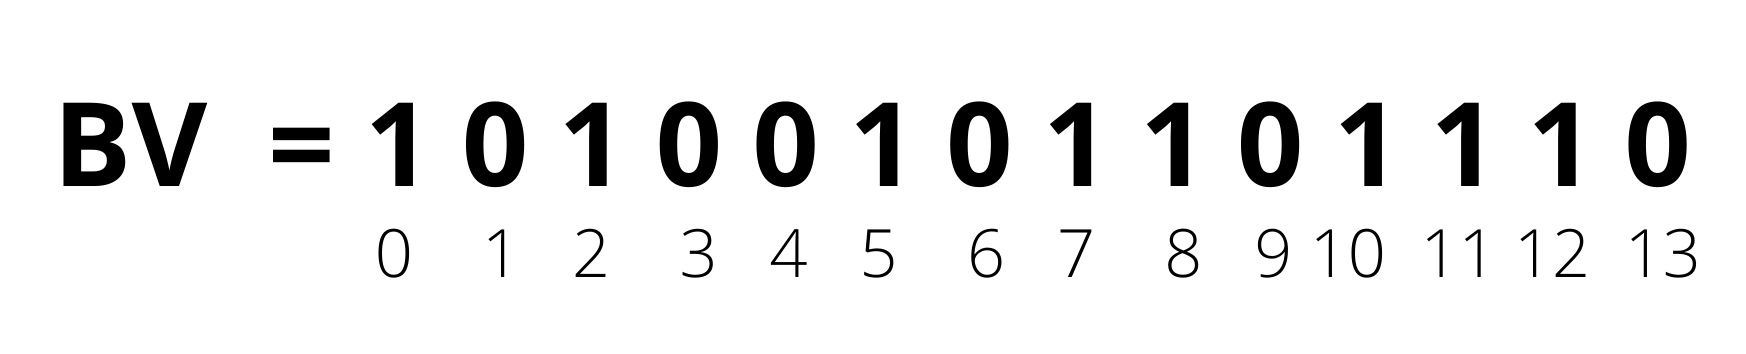
\includegraphics[scale=0.5]{images/bitvector.png}
            \end{figure} 
        \end{itemize}
    \end{frame}
    
    \begin{frame}{Vetores de bits - access}
        Exemplo: $access(BV,10)=1$
        \begin{figure}[h!]
            \centering
            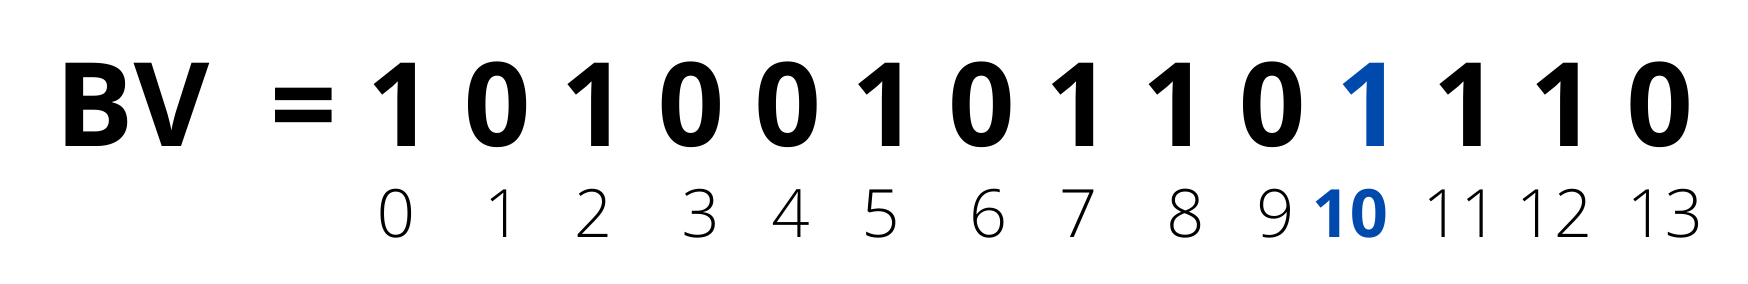
\includegraphics[scale=0.7]{images/access-res.png}
        \end{figure} 
    \end{frame}
    
    
    \begin{frame}{Vetores de bits - rank}
    Sequência de $n$ elementos sobre o alfabeto $\Sigma = \{0,1\}$, no qual podem ser realizadas as seguintes operações \citep{book-compact-data-structures}:
        \vspace{0.5cm}
        \begin{itemize} 
            \item $rank_v(BV,i)$: seja $v \in \{0,1\}$, e $0 \leq i < n$, retorna o número de ocorrências de $v$ no intervalo $BV[0,i]$.
            \vspace{0.5cm}
            
            Exemplo: $rank_0(BV,8)$
            
            \begin{figure}[h!]
                \centering
                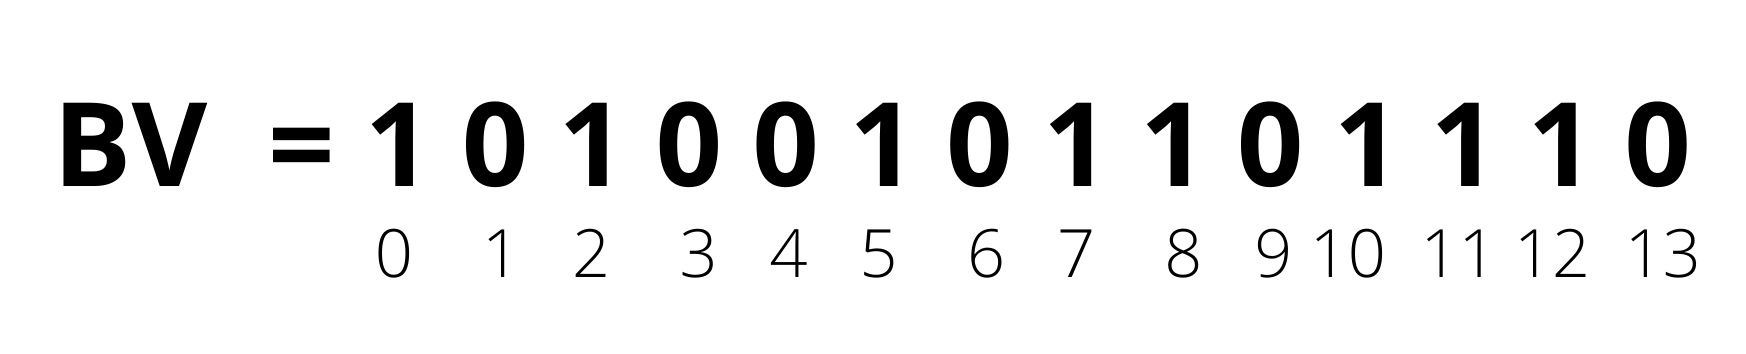
\includegraphics[scale=0.5]{images/bitvector.png}
            \end{figure} 
        \end{itemize}
    \end{frame}
    
    \begin{frame}{Vetores de bits - rank}
        Exemplo: $rank_0(BV,8)=4$
        \begin{figure}[h!]
            \centering
            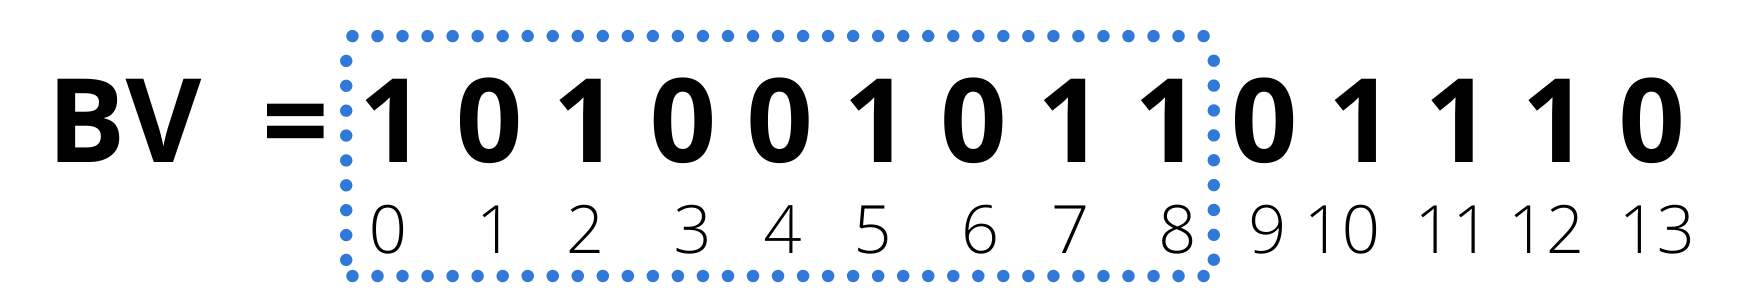
\includegraphics[scale=0.7]{images/rank-res.png}
        \end{figure} 
    \end{frame}
    
    \begin{frame}{Vetores de bits - select}
    Sequência de $n$ elementos sobre o alfabeto $\Sigma = \{0,1\}$, no qual podem ser realizadas as seguintes operações \citep{book-compact-data-structures}:
        \vspace{0.5cm}
        \begin{itemize} 
              \item $select_v(BV,i)$: dado $v \in \{0,1\}$ e $i \geq 0$, retorna a posição do i-ésimo bit $v$ em $BV[0,n-1]$.
              \vspace{0.5cm}
            
                Exemplo: $select_1(BV,7)$
            
                \begin{figure}[h!]
                    \centering
                    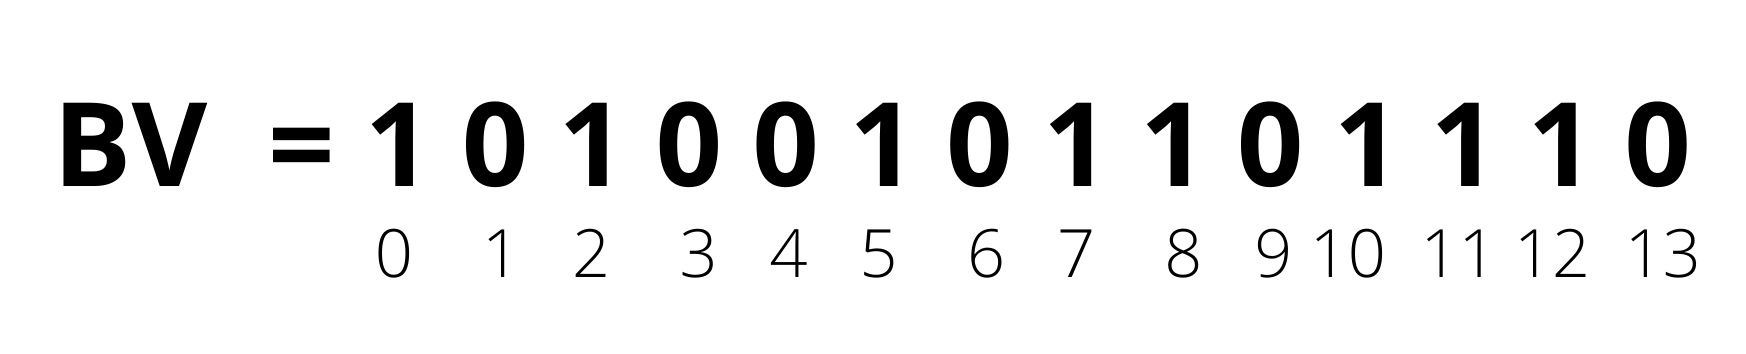
\includegraphics[scale=0.5]{images/bitvector.png}
                \end{figure} 
        \end{itemize}
    \end{frame}
    
    \begin{frame}{Vetores de bits - select}
        Exemplo: $select_1(BV,7)=12$
        \begin{figure}[h!]
            \centering
            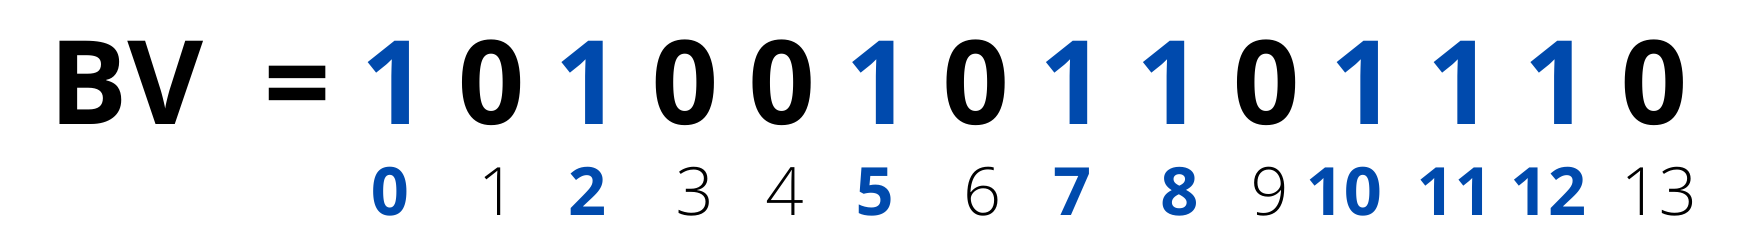
\includegraphics[scale=0.7]{images/select-res.png}
        \end{figure} 
    \end{frame}

\begin{frame}{Representações sucintas de árvores}
\begin{itemize}
    \item Parênteses balanceados (BP);
    \item Depth-First Unary Degree Sequence (DFUDS);
    \item Level-order Unary Degree Sequence (LOUDS);
\end{itemize}    
\end{frame}

\begin{frame}{Representações sucintas de árvores}
    \textbf{Representação de árvores sucintas via Parênteses Balanceados}
        \begin{figure}[h!]
            \centering
            
            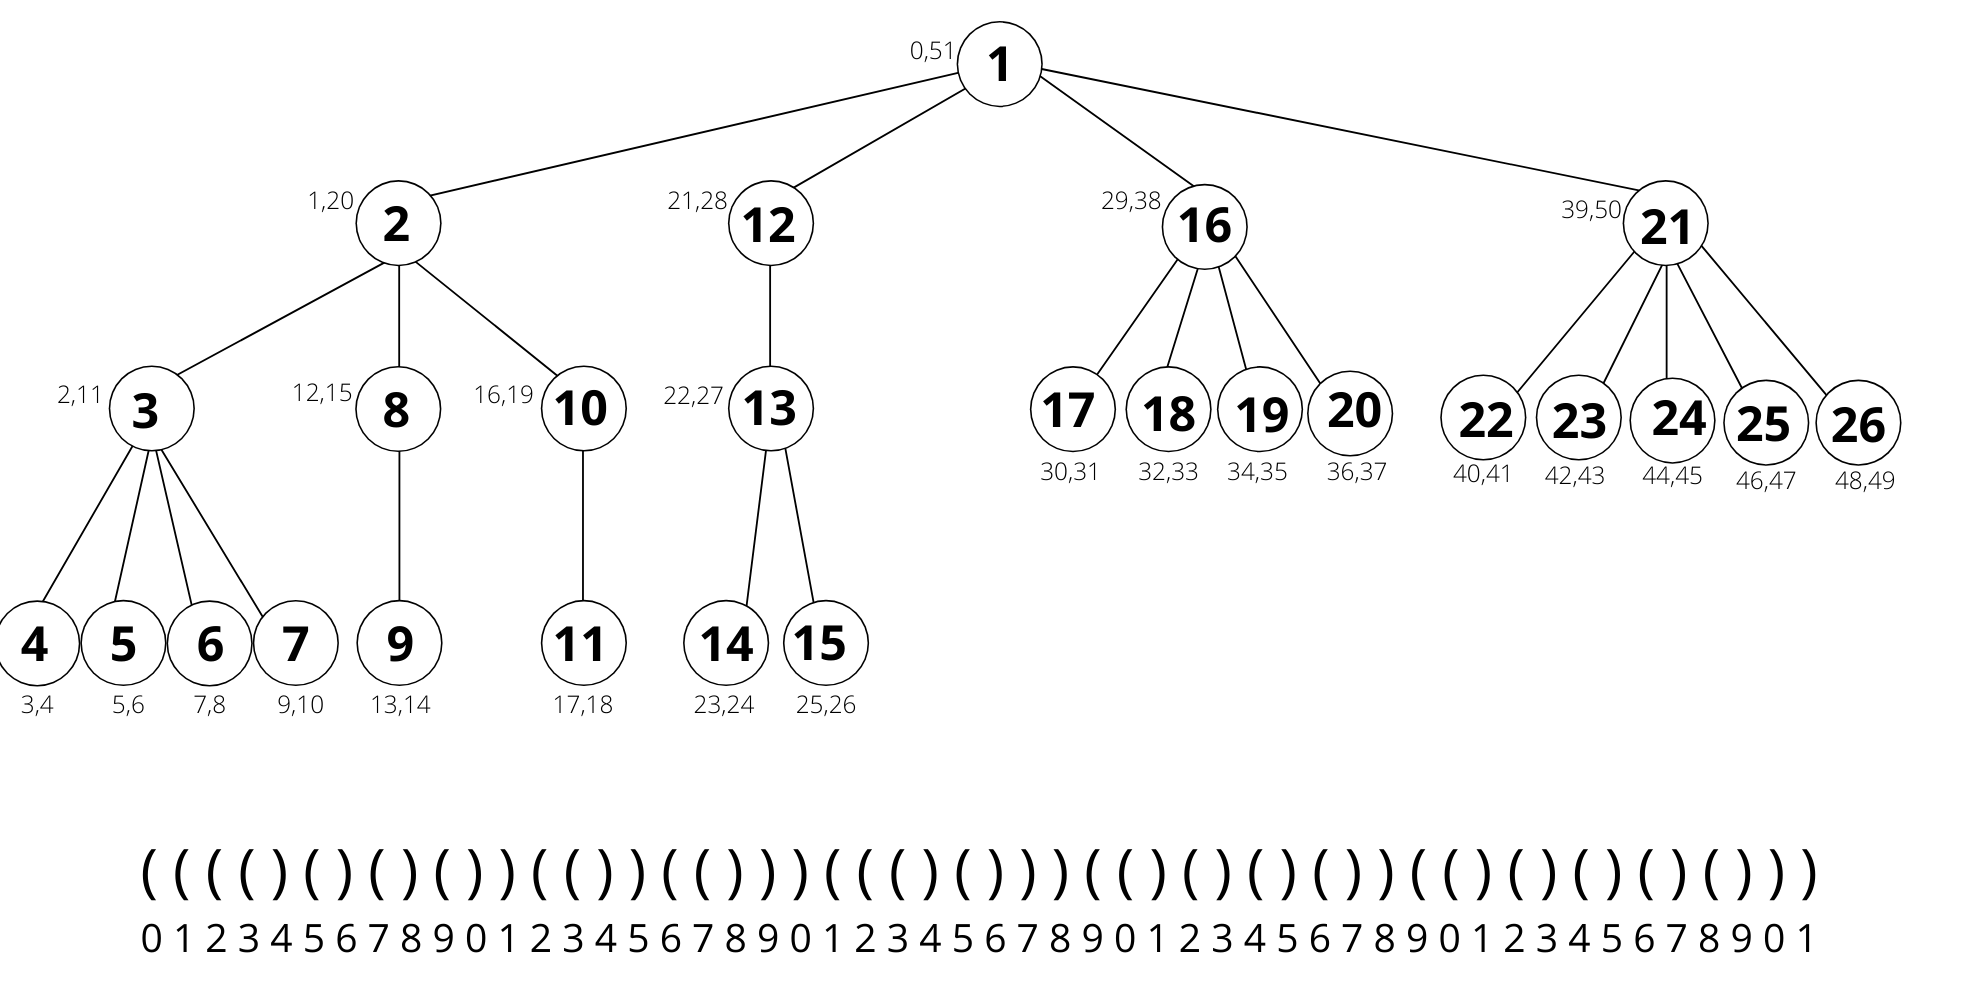
\includegraphics[scale=0.37]{images/arvore_geral.png}
        \end{figure} 
\end{frame}

\begin{frame}{Representações sucintas de árvores}
    \textbf{Representação de árvores sucintas via parênteses balanceados}
        \begin{itemize}
            \item Sequência de $2n$ parênteses balanceados;
            \item Complexidade de espaço $2n + o(n)$ bits;
            \item Através de estruturas auxiliares suporta:
            \begin{itemize}
                \item findclose(B,i);
                \item findopen(B,i);
                \item excess(B,i);
            \end{itemize}
        \end{itemize}
    \end{frame}
    
    \begin{frame}{Representações sucintas de árvores}
    Exemplo: \textit{excess(B,6) = -1}
        \begin{figure}[h!]
            \centering
            
            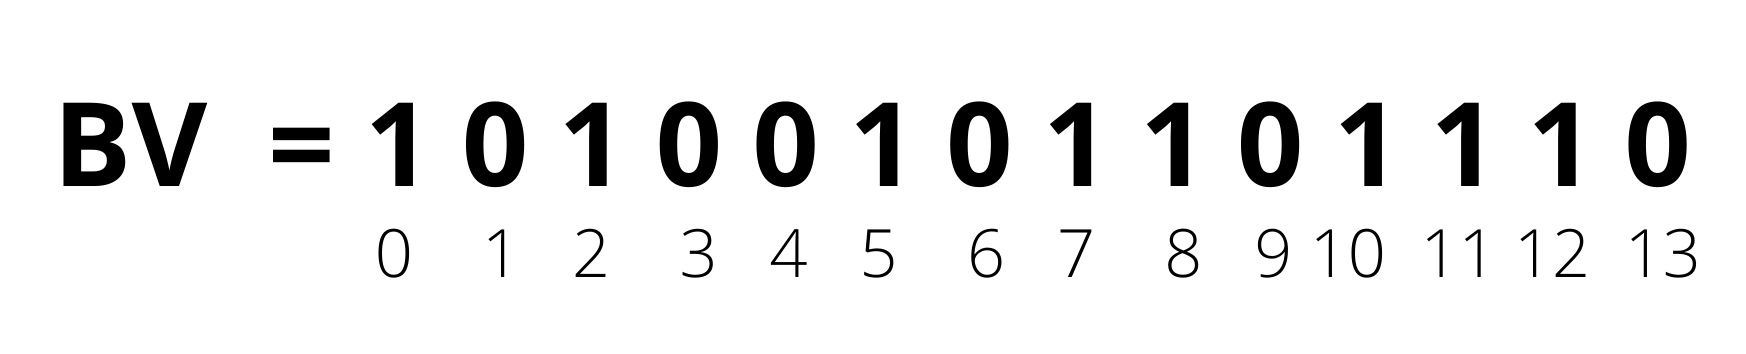
\includegraphics[scale=0.5]{images/bitvector.png}
        \end{figure} 
\end{frame}
\begin{frame}{Representações sucintas de árvores}
    \textbf{Representação de árvores sucintas via DFUDS}
        \begin{figure}[h!]
            \centering
            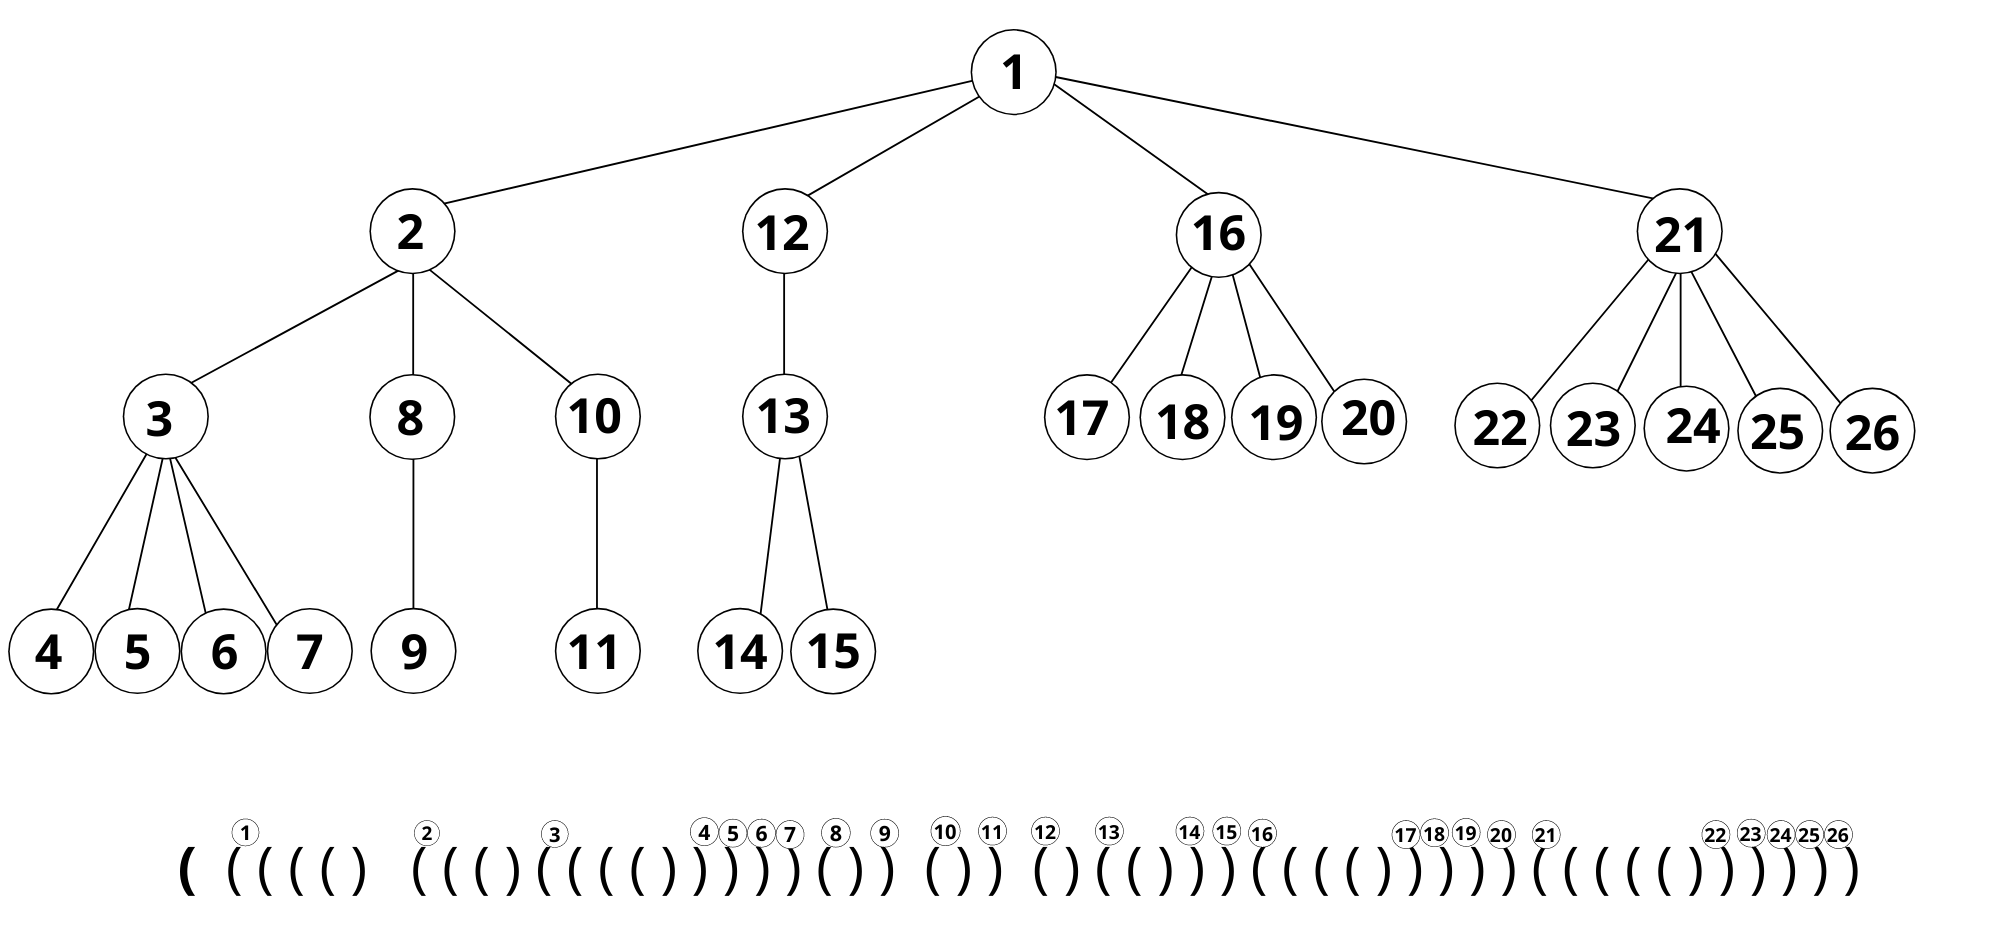
\includegraphics[scale=0.37]{images/dfuds.png}
        \end{figure} 
\end{frame}
\begin{frame}{Representações sucintas de árvores}
    \textbf{Representação de árvores sucintas via LOUDS}
        \begin{figure}[h!]
            \centering
            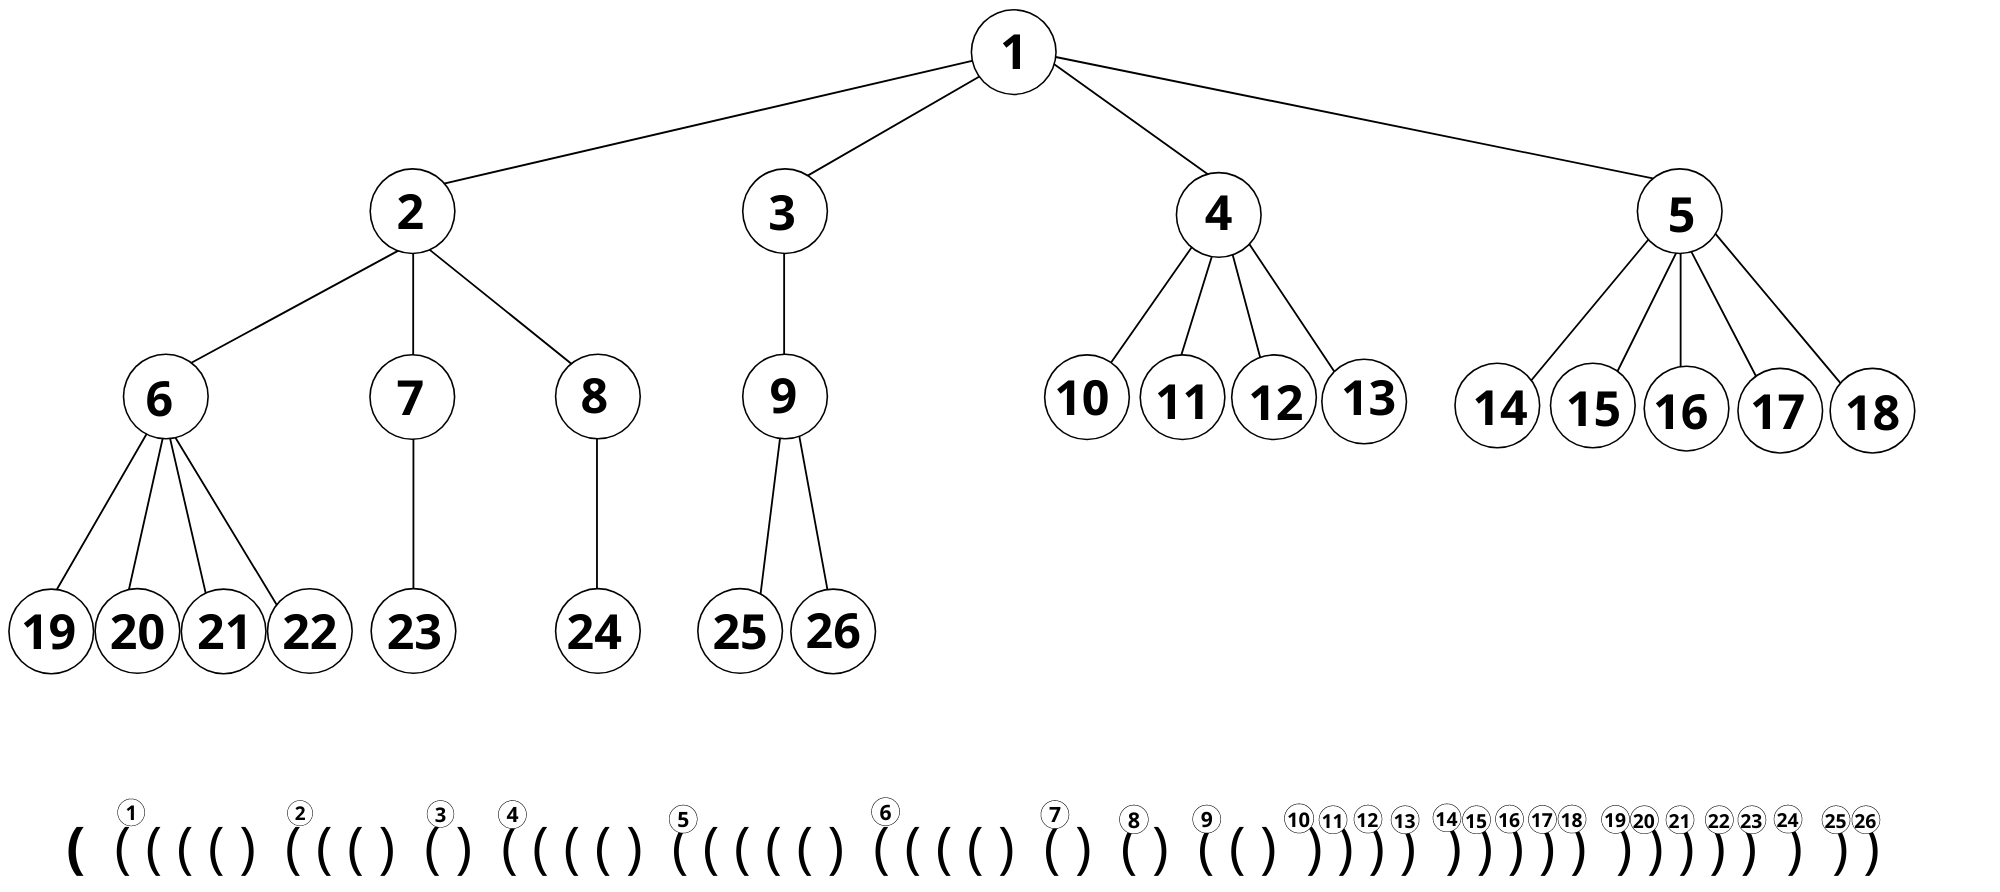
\includegraphics[scale=0.37]{images/louds.png}
        \end{figure} 
\end{frame}



\begin{frame}{range min-Max tree (rmM-tree)}
    \begin{itemize}
        \item Construção bottom-up;
        \item Árvore binária completa, baseada em intervalos de tamanho $b$;
        \item Cada nó cobre valores de excessos dentro de um intervalo;
        \item Complexidade de espaço igual à $n + O(\frac{n}{b} \log n)$ bits;
        \item Operações realizadas em tempo $O(\log n)$.
    \end{itemize}
\end{frame}

\begin{frame}{range min-Max tree binária}
    \begin{figure}[h!]
        \centering
        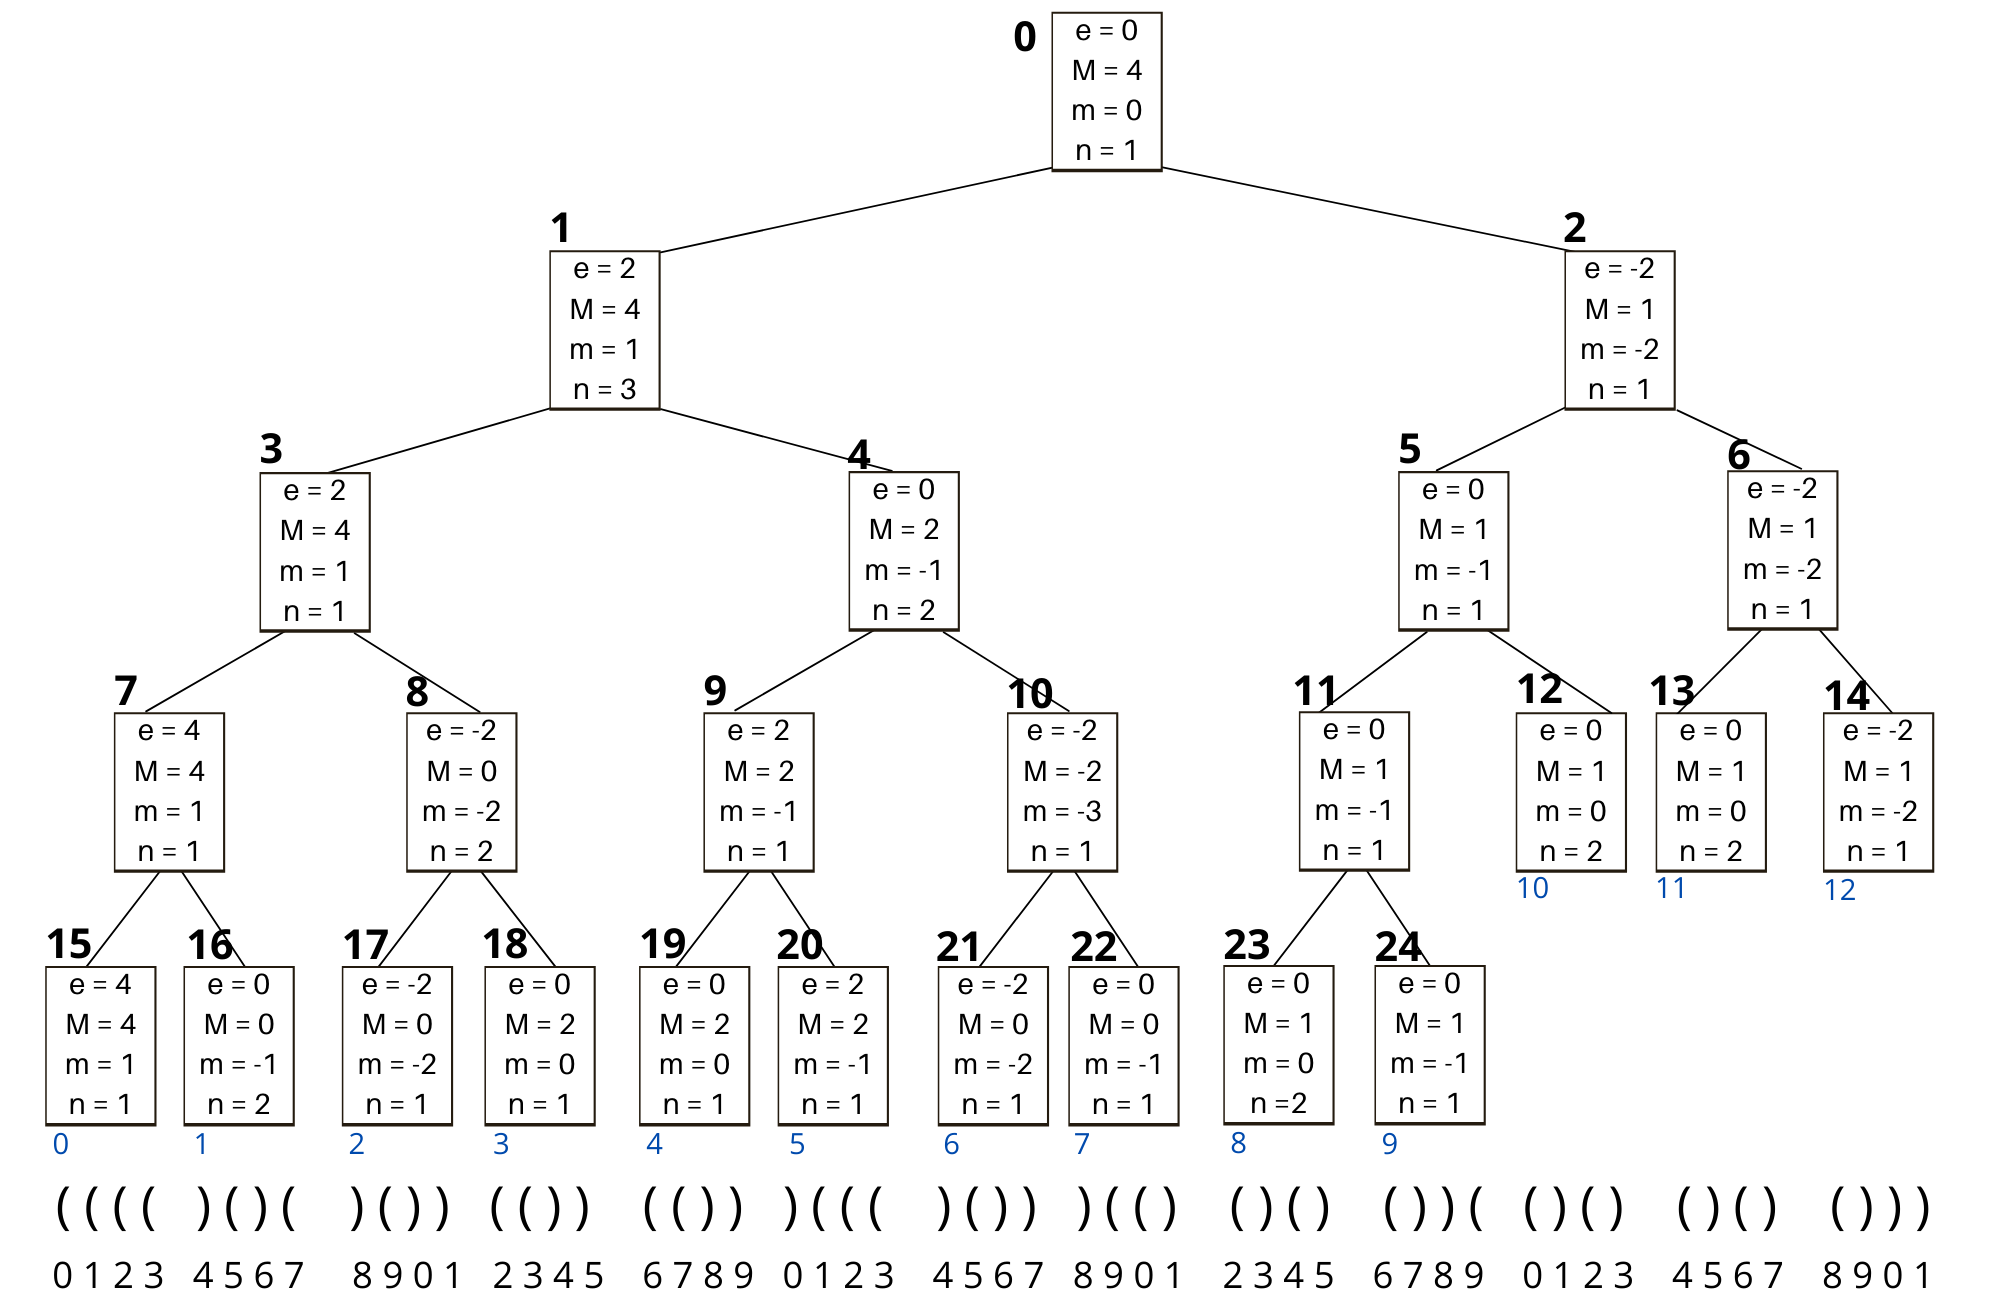
\includegraphics[scale=0.3]{images/rmm-tree-bin.png}\\
        \caption{rmM-tree binária com blocos de tamanho 4}
    \end{figure} 
\end{frame}

\begin{frame}{rmM-tree: Registros}

    \textbf{Valores de excesso}
        Dado um nó $v$ que cobre um intervalo $BP[s,e]$, então:
        \begin{itemize}
            \item $R[v].e$: excesso total no intervalo\\
            $R[v].e = excess(e)-excess(s-1)$.
            \item $R[v].M$: excesso máximo no intervalo\\
            $R[v].M = \max\{excess(i) - excess(s - 1) | s \leq i \leq e\}$.
            \item $R[v].m$: excesso mínimo no intervalo\\
            $R[v].m = \min\{excess(i) - excess(s - 1) | s \leq i \leq e\}$.
            \item $R[v].n$: número de vezes que o excesso mínimo ocorre no intervalo\\
            $R[v].n = |\{BP[i]=R[v].m | s \leq i \leq e\}|$.
        \end{itemize}
\end{frame}

\begin{frame}{rmM-tree: Registros}
    \textbf{Nós internos e raíz}
    \begin{figure}[h]
        \begin{minipage}[c]{0.35\linewidth}
            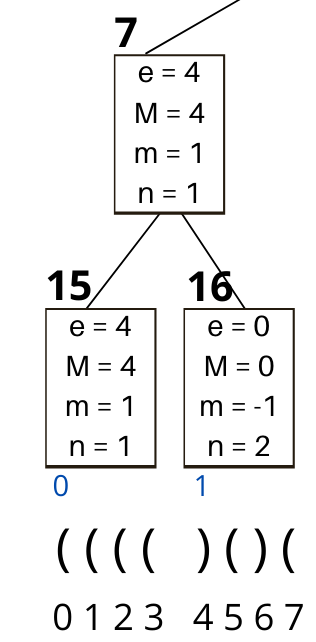
\includegraphics[scale=0.65]{images/internal-nodo.png}
        \end{minipage}
        \begin{minipage}[c]{0.49\linewidth}
            \begin{tabular}{l}\\
                R[7].e = R[15].e +  R[16].e.             \\
                R[7].M=max(R[15].M, R[15].e+ R[16].M).\\
                R[7].m=min(R[15].m, R[15].e+ R[16].m). \\
                R[7].n= R[15].n. \\
            \end{tabular}
        \end{minipage}
    \end{figure}
\end{frame}

\begin{frame}{rmM-tree: Operações}
    \begin{table}[]
       \begin{tabular}{|c|c|c|}
            \hline
            \multicolumn{3}{|c|}{\textbf{Operações}}  \\ \hline  
            fwdsearch(i,d)                       &bwdsearch(i,d)                        &minExcess(i,j) \\ \hline               
            maxExcess(i,j)                       & minSelectExcess(i,j,t)               & minCount(i,j)                       \\ \hline
            enclose(i)                           & rank\_v(i)                           & select\_v(i)                         \\ \hline                                
            findClose(i)                         & findOpen(i)                          & rmq(i,j) \\ \hline
            inspect(i)                           & preRank(i)                           & postRank(i)                    \\ \hline
            preSelect(i)                         & postSelect(i)                        & isLeaf(i)                       \\ \hline
            isAncestor(i,j)                      & depth(i)                             & parent(i)   \\ \hline
        \end{tabular}
    \end{table}
\end{frame}

\begin{frame}{rmM-tree: Operações}
    \begin{table}[]
        \begin{tabular}{|c|c|c|}
        \hline
        \multicolumn{3}{|c|}{\textbf{Operações}}                                                         \\ \hline
        firstChild(i) &  lastChild(i) & nextSibling(i) \\ \hline
        prevSibling(i)    & subtreeSize(i)                   & levelAncestor(i,d)         \\ \hline
        \multicolumn{1}{|c|}{level-next(i)} & levelPrev(i)  & \multicolumn{1}{c|}{levelLmost(d)} \\ \hline
        levelRmost(d)                      & lca(i,j)       & deepestNode(i)                     \\ \hline
        degree(i)                           & child(i,q)     & childRank(i)                       \\ \hline
        leafRank(i)                        & leafSelect(i) & lmostLeaf(i)                       \\ \hline
        \end{tabular}
    \end{table}
\end{frame}


\begin{frame}{rmM-tree: operações}
    Problema: Dado um nó codificado em $i=1$, encontrar o nó codificado em $j>i$, mais à esquerda de $i$.

    Solução: 
    $$nextSibling(i) = findClose(i) +1$$ 
    $$findClose(i) = fwdSearch(i,-1)$$ 
 \end{frame}

 \begin{frame}{rmM-tree: $nextSibling$}
    Problema: Computar $nextSibling(1)$.
     \begin{figure}[h!]
         \centering
         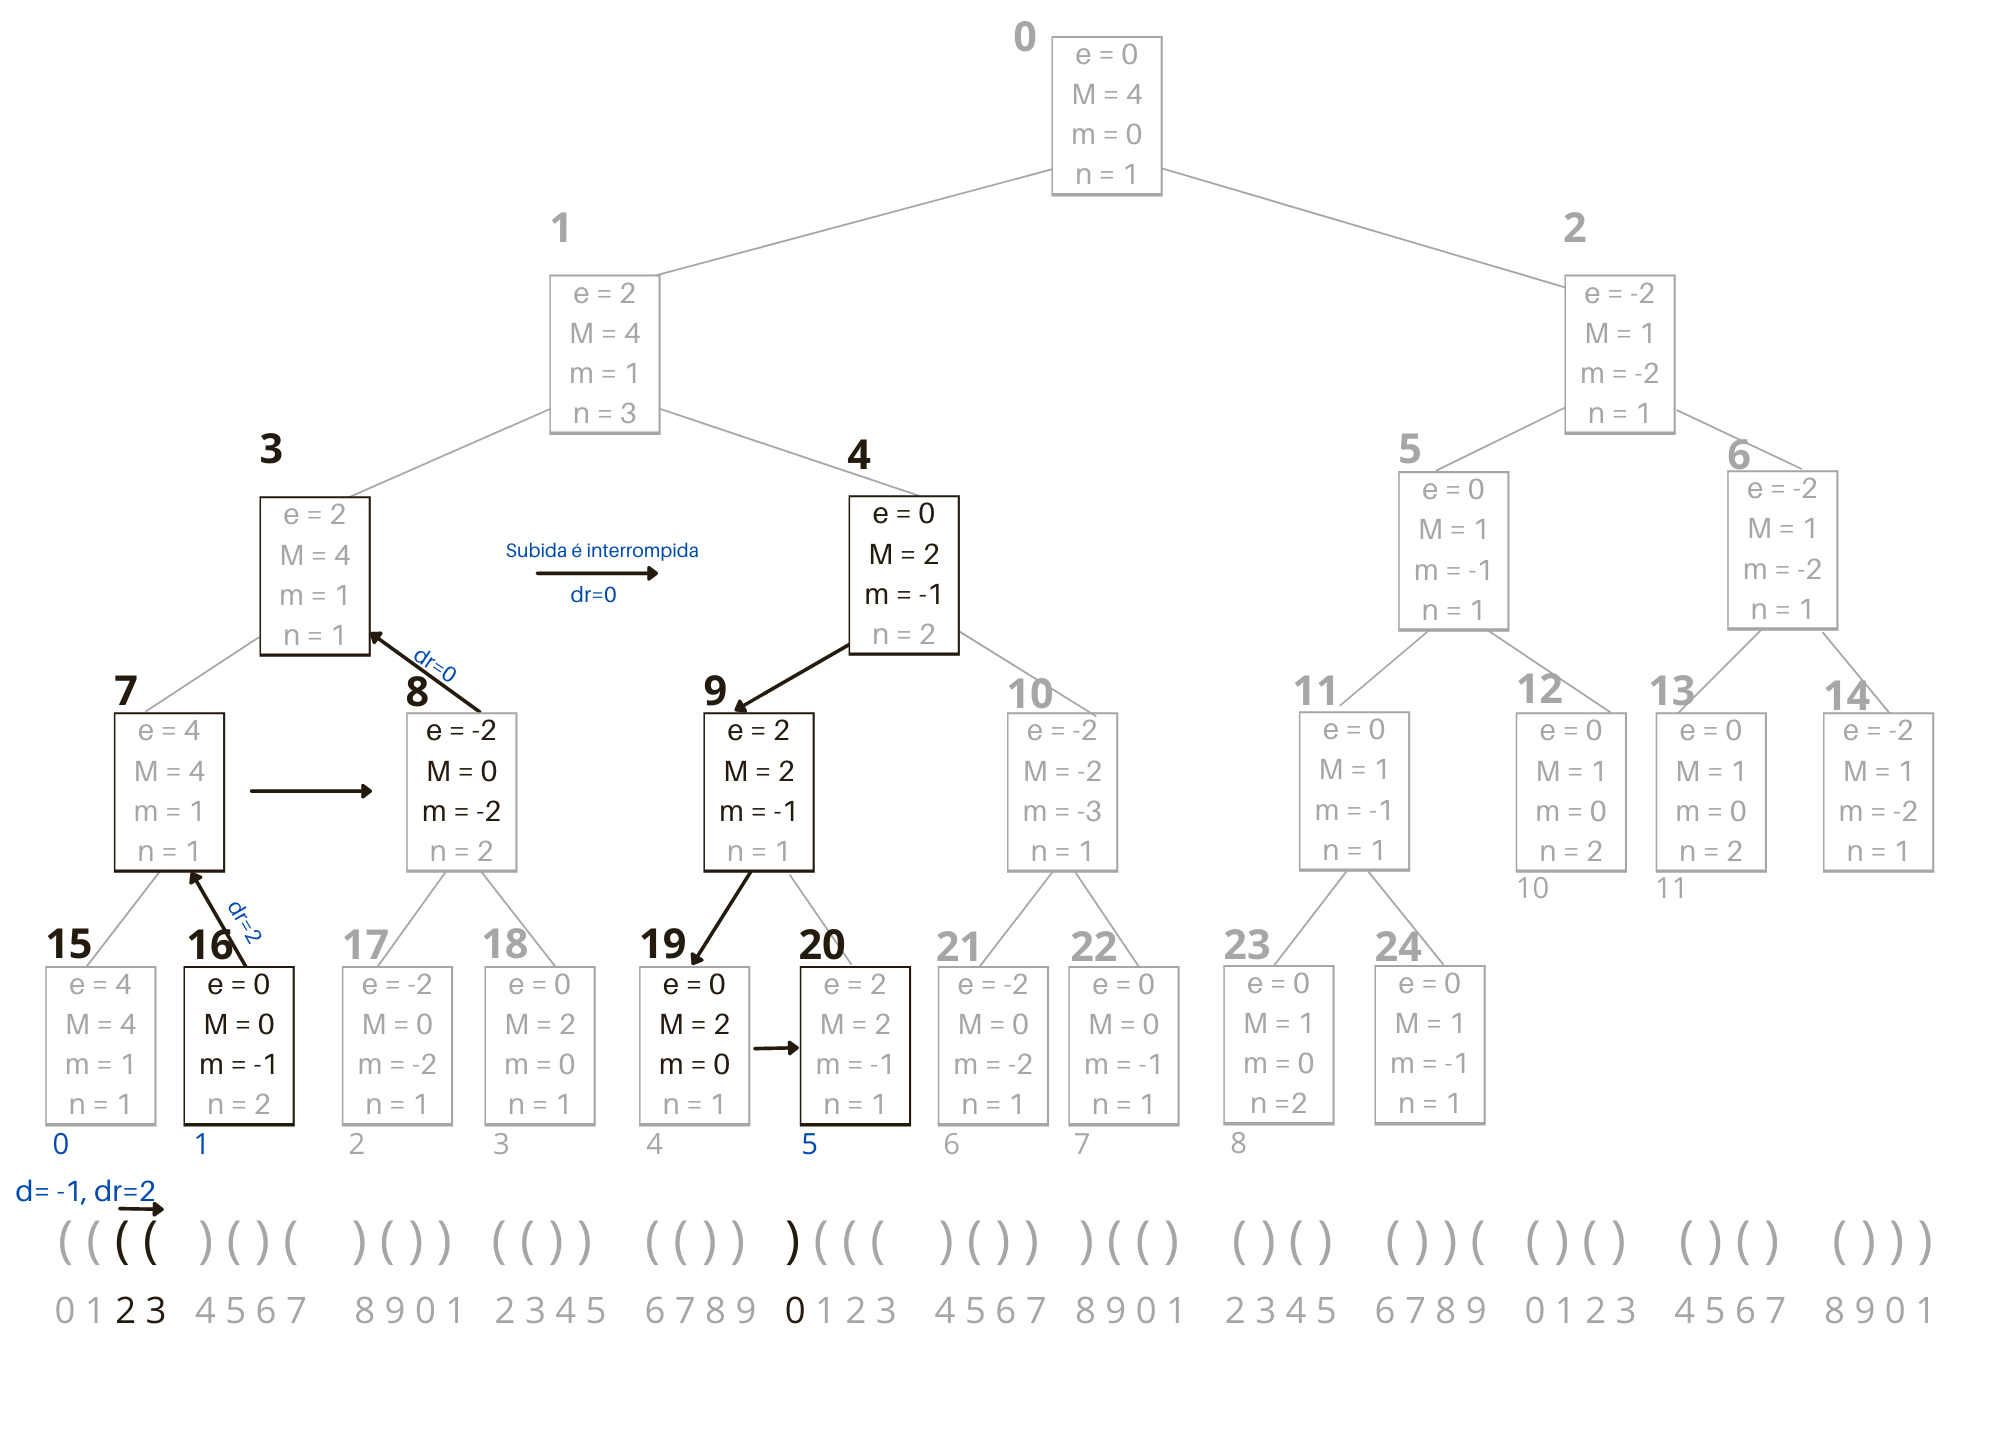
\includegraphics[scale=0.27]{images/rmm-tree-bin-fwdSearch.png}\\
         \caption{Simulação de $fwdSearch(1,-1)=20$}
     \end{figure} 
 \end{frame}

 \begin{frame}{rmM-tree: $nextSibling$}
    Problema: Dado um nó codificado em $i=1$, encontrar o nó codificado em $j>i$, mais à esquerda de $i$.

    Solução: 
    $$findClose(1) = fwdSearch(1,-1) = 20 $$ 
    $$nextSibling(1) = fwdSearch(1,-1) + 1 = 21 $$ 
 \end{frame}

 \begin{frame}{rmM-tree: $nextSibling$}
    Solução:  $nextSibling(1)$.
     \begin{figure}[h!]
         \centering
         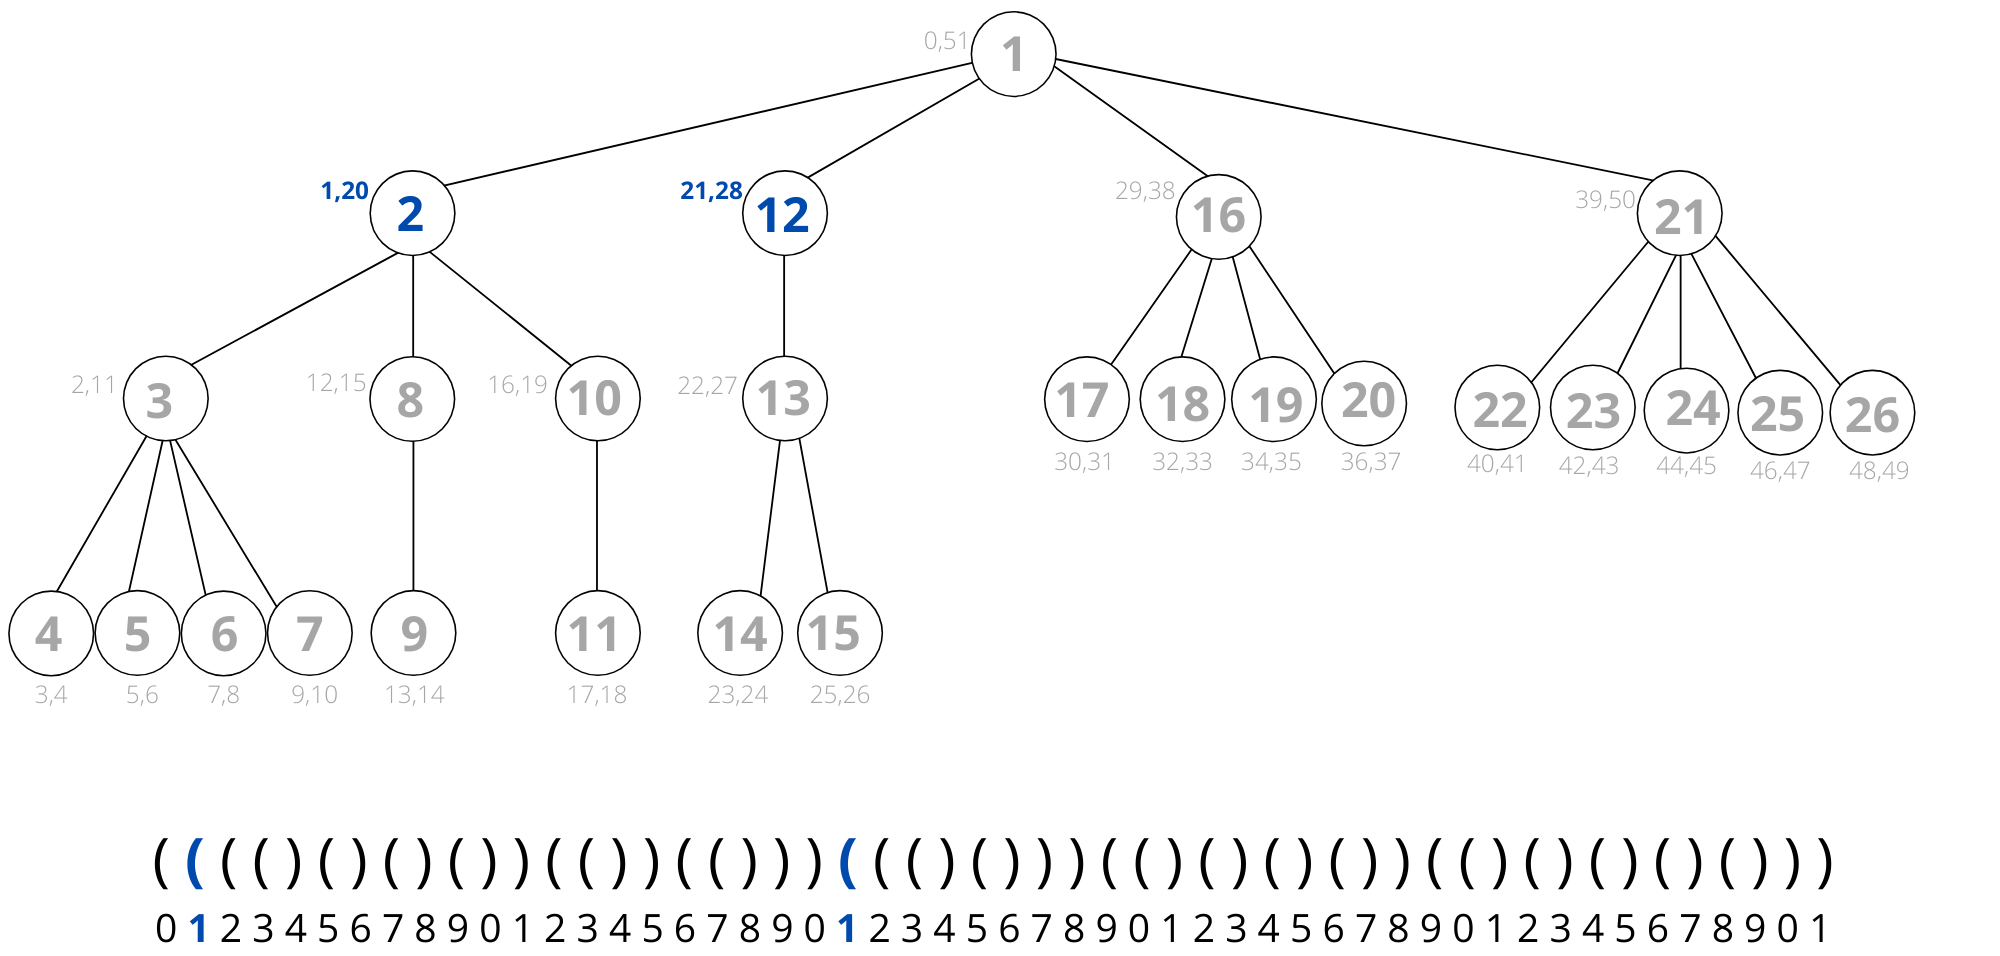
\includegraphics[scale=0.40]{images/nextSibling-res.png}\\
         \caption{Árvore de entrada}
     \end{figure} 
 \end{frame}

\begin{frame}{rmM-tree: operações}
    Problema: Verificar o ancestral comum mais baixo dos nós codificados em $i=5$ e $j=17$.
     \begin{figure}[h!]
         \centering
         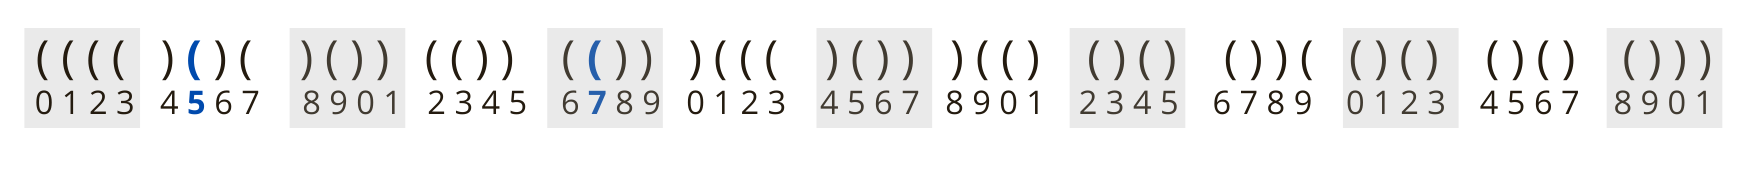
\includegraphics[scale=0.7]{images/bp-sequence.png}\\
         \caption{Sequência de parênteses balanceados, representando uma árvore $T$}
     \end{figure} 
 
 \end{frame}

 \begin{frame}{rmM-tree: $lca$}
    Problema: Verificar o ancestral comum mais baixo dos nós codificados em $i=5$ e $j=17$.

    Solução: 
    $$lca(i,j) = 
    \begin{cases}
          i,  \mbox{se } isAncestor(i,j); \\
         j, \mbox{se } isAncestor(j,i); \\
         parent(rmq(i ,j)+1)
    \end{cases}
    $$ 
 \end{frame}

 \begin{frame}{rmM-tree: $lca$}
    Problema: Verificar o ancestral comum (mais baixo) dos nós codificados em $i=5$ e $j=17$.


    Solução:\\
    \begin{itemize}
        \item \textit{isAncestor(,i,j)} verifica se o nó codificado em $i$ é ancestral do nó $j$;
        \item O mesmo vale para \textit{isAncestor(j,i)};
        \item Usar o terceiro caso.
    \end{itemize}
 \end{frame}


 \begin{frame}{rmM-tree: $lca$}
    Problema: Computar $lca(5,17)$.


    Solução: $ parent(rmq(i ,j)+1)$\\
    \begin{itemize}
        \item $rmq(i,j) = fwdSearch(i-1, minExcess(i,j))$;
        \item $parent(rmq(i,j)+1) = bwdSearch(rmq(i,j)+1, 0) + 1$.
    \end{itemize}
 \end{frame}


\begin{frame}{rmM-tree: $lca$}
    Problema: Computar $lca(5,17)$.
     \begin{figure}[h!]
         \centering
         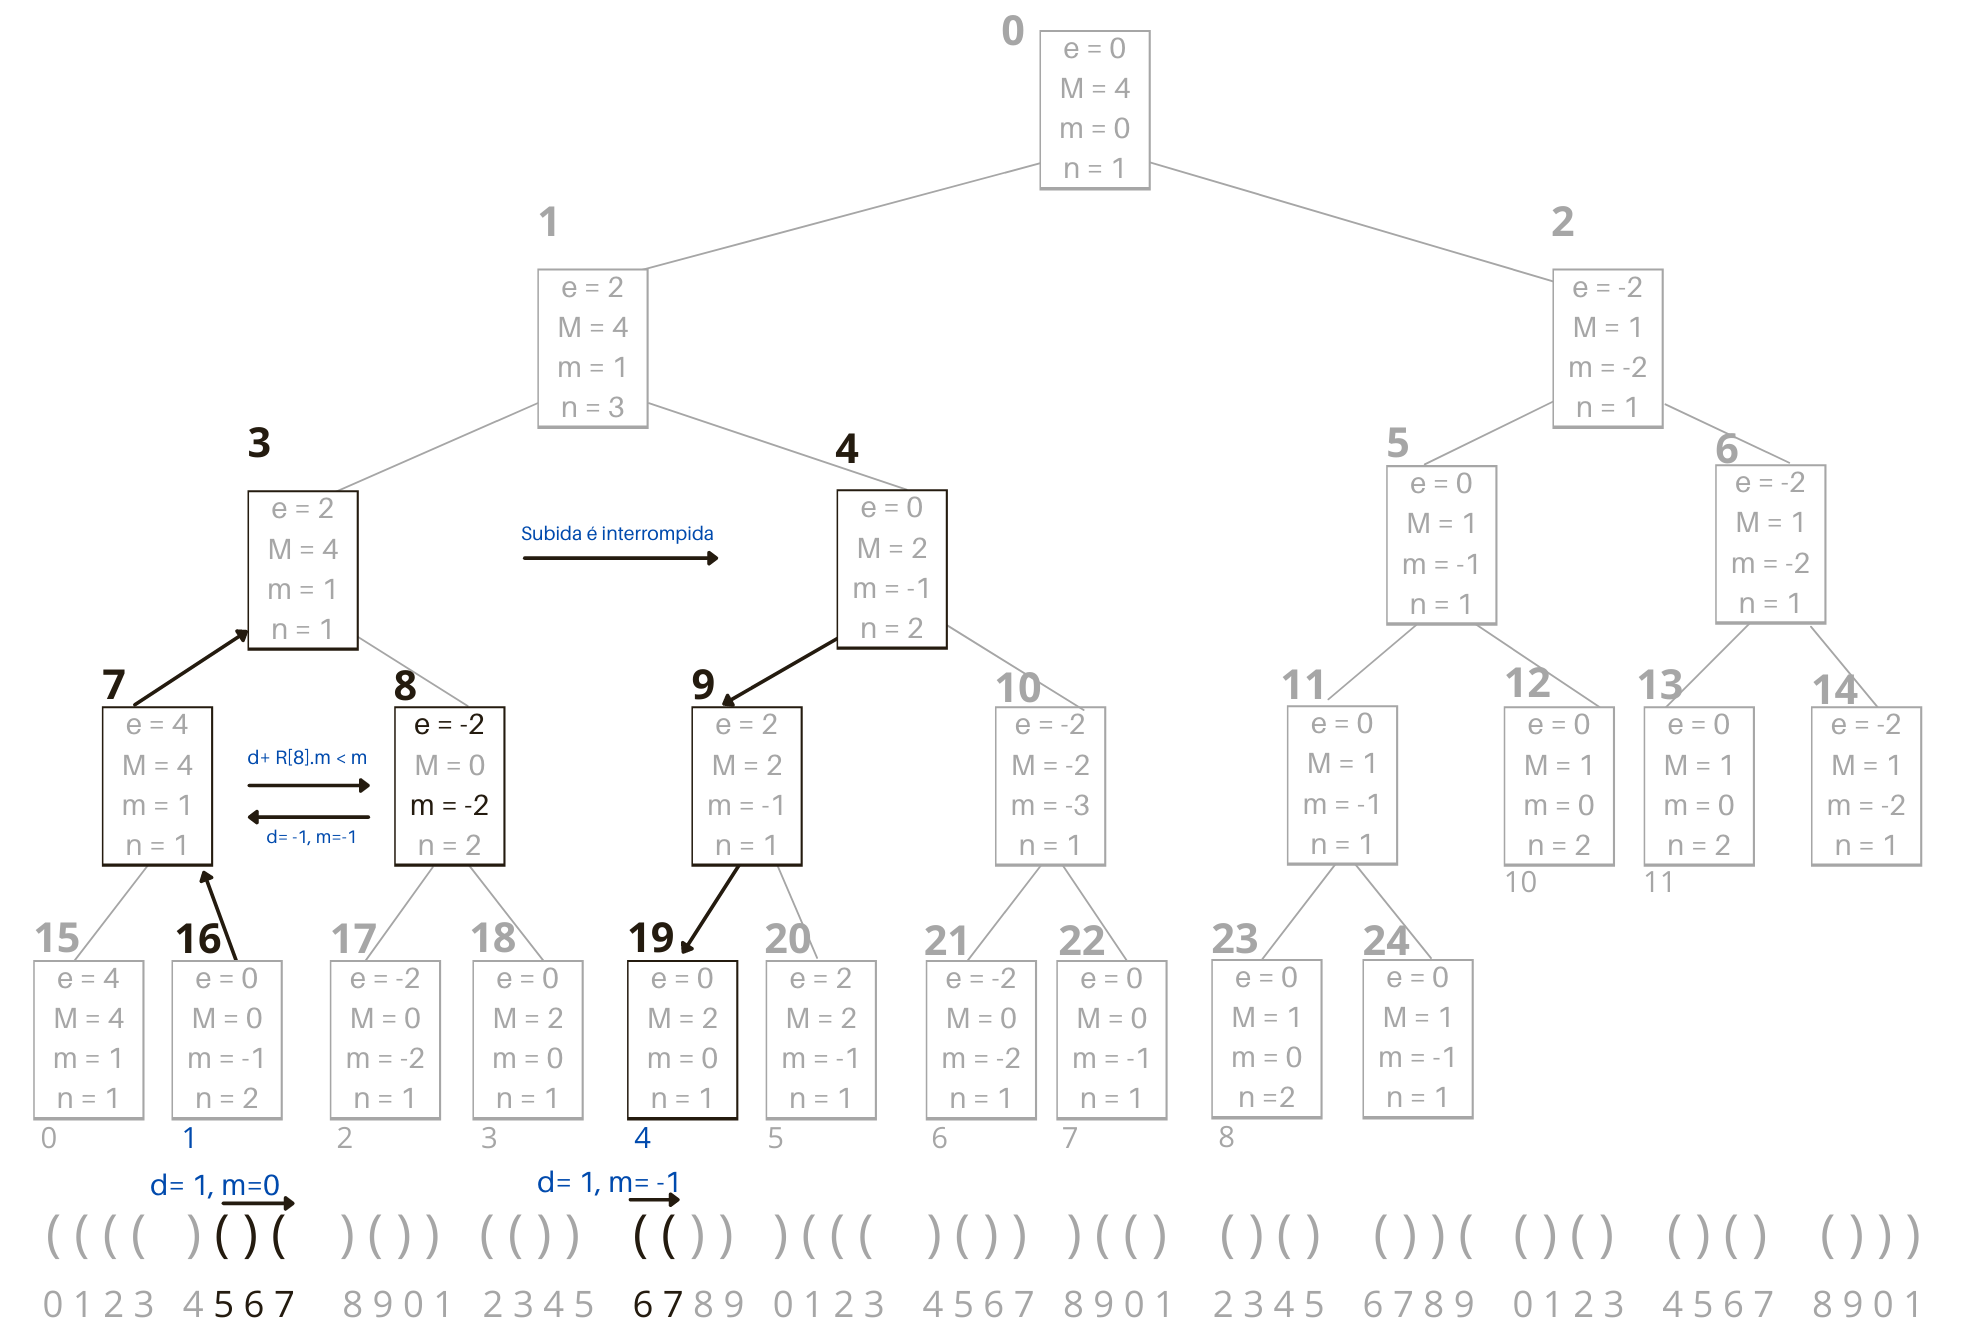
\includegraphics[scale=0.27]{images/rmm-tree-bin-minexcess.png}\\
         \caption{Simulação de $minExcess(5,17)=-1$}
     \end{figure} 
 \end{frame}


% \begin{frame}{rmM-tree: operações}
%     Problema: Computar $lca(5,17)$.
%      \begin{figure}[h!]
%          \centering
%          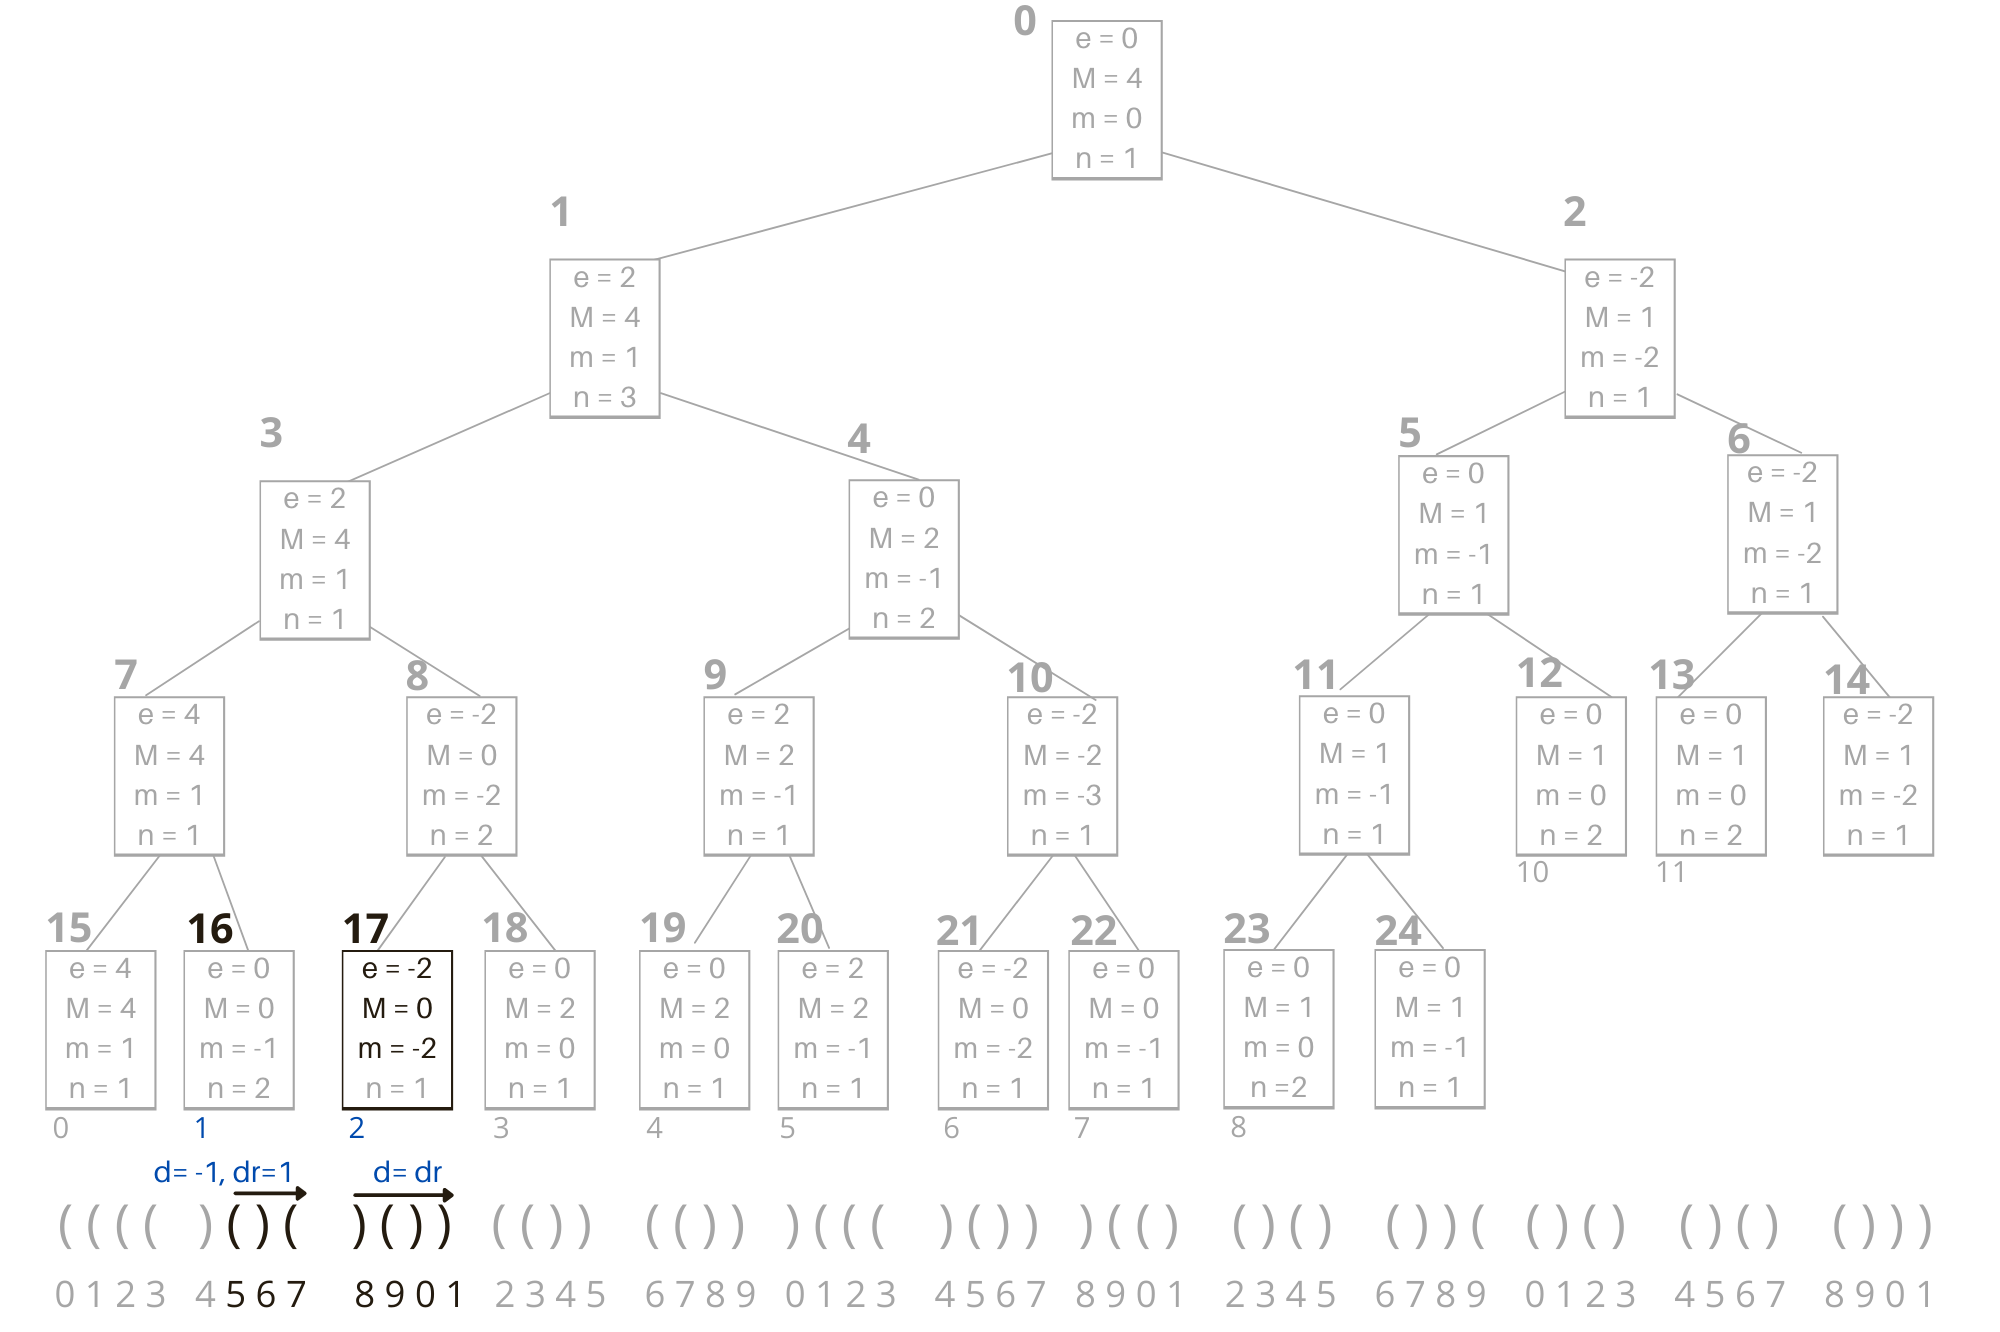
\includegraphics[scale=0.27]{images/rmm-tree-bin-fwd-lca.png}\\
%          \caption{Simulação de $fwdSearch(4,-1)=11$}
%      \end{figure} 
%  \end{frame}

 \begin{frame}{rmM-tree: $lca$}
    Solução: Computar $lca(5,17)$.
     \begin{figure}[h!]
         \centering
         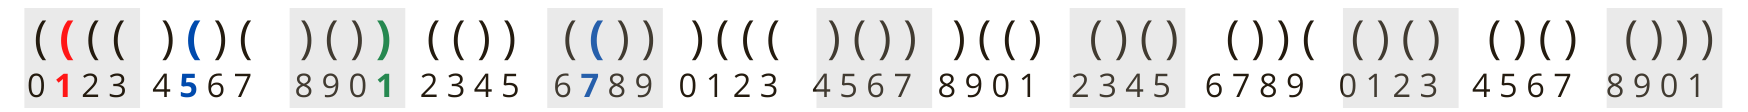
\includegraphics[scale=0.8]{images/lca-resposta.png}\\
         \caption{Nós acessados durante a operação $lca(5,17)$}
     \end{figure} 
 \end{frame}

 \begin{frame}{rmM-tree: $lca$}
    Solução: Computar $lca(5,17)$.
     \begin{figure}[h!]
         \centering
         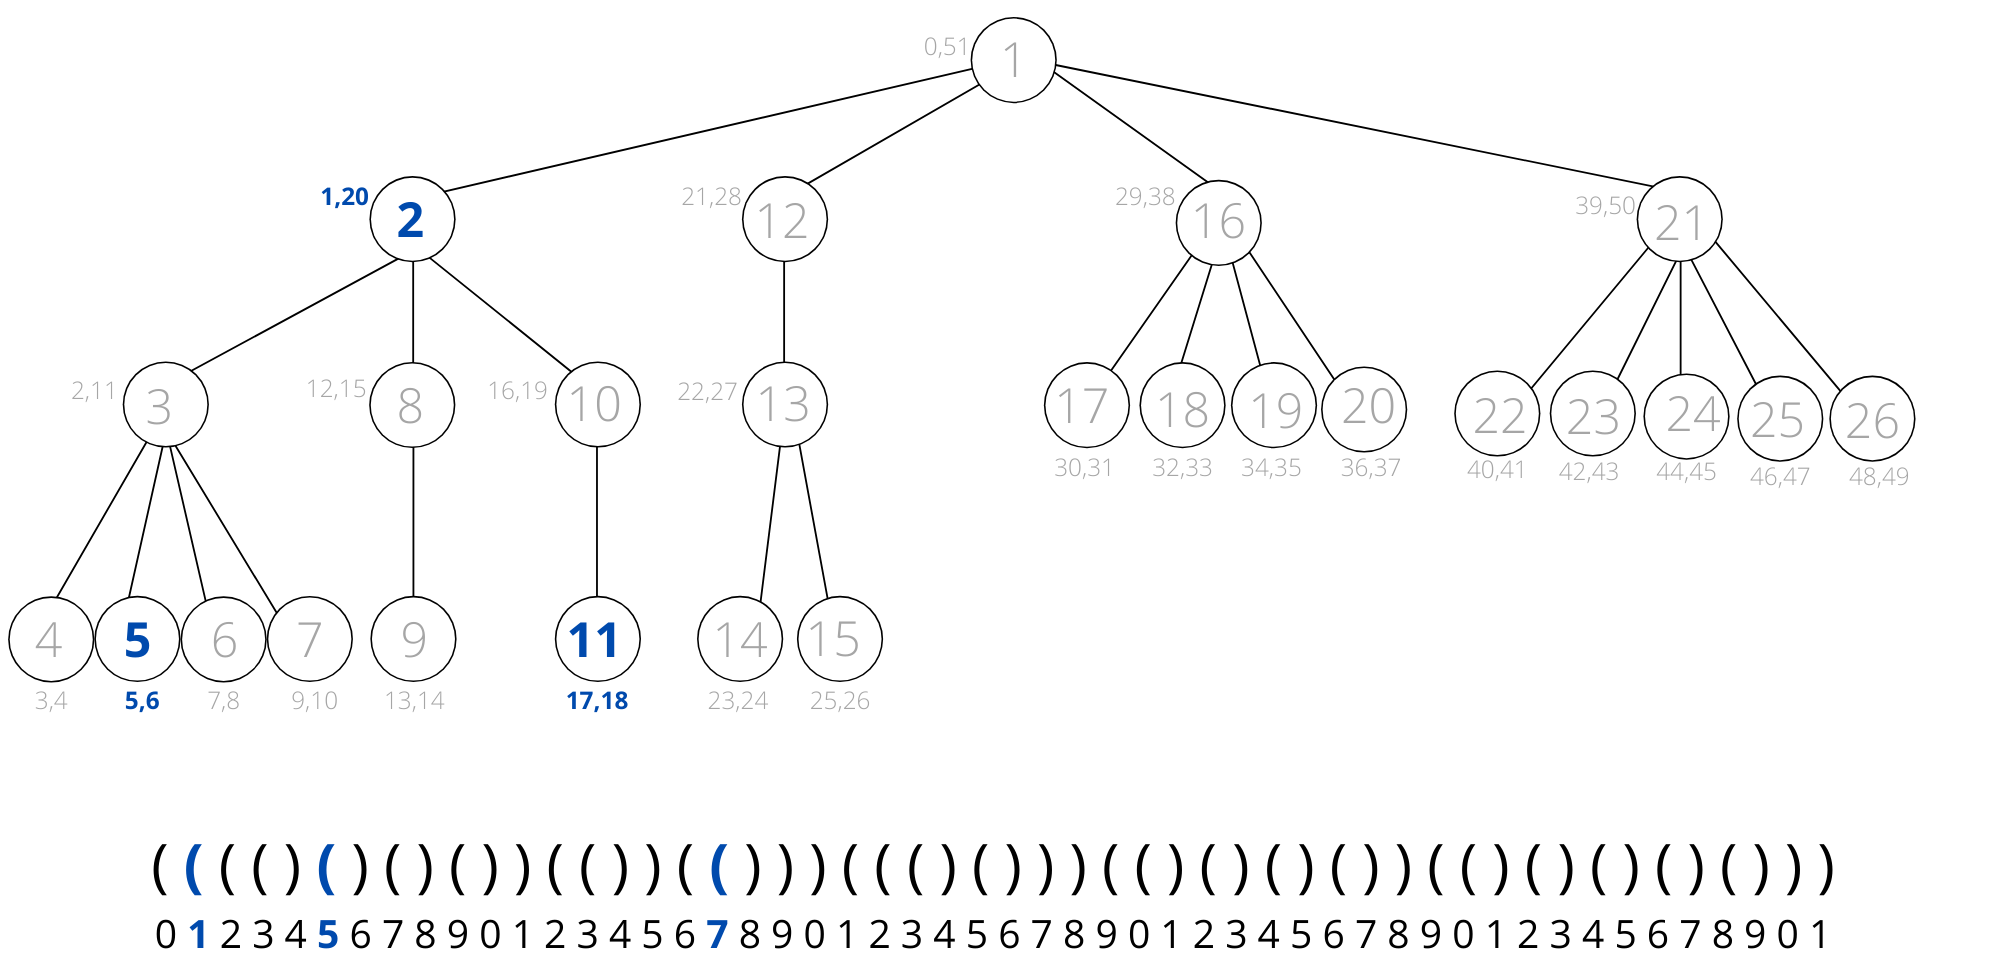
\includegraphics[scale=0.40]{images/lca-res.png}\\
         \caption{Árvore de entrada}
     \end{figure} 
 \end{frame}

\begin{frame}{Aproveitamento de cache}
    \begin{itemize}
        \item Expansão da memória principal;
        \item Dados residindo em memória principal: um novo gargalo;
        \item Falhas de cache.
    \end{itemize}
\end{frame}

\begin{frame}{Aproveitamento de cache}
    \begin{itemize}
        \item Maximização da quantidade de informação em um nó \cite{paper-effect-node-size-cache-b-trees}:
        \begin{itemize}
            \item Altura da árvore;
            \item Linha de cache.
        \end{itemize}
        \item Fator de ramificação \cite{paper-making-btree-cache}:
        \begin{itemize}
            \item Cache Sensitive Tree (CSS-tree);
            \item Cache Sensitive B$^+$-Tree (CS$B^+$-tree);
            \item Árvores B$^+$.
        \end{itemize}
    \end{itemize}
\end{frame}